%% Based on a TeXnicCenter-Template by Tino Weinkauf.
%%%%%%%%%%%%%%%%%%%%%%%%%%%%%%%%%%%%%%%%%%%%%%%%%%%%%%%%%%%%%

%%%%%%%%%%%%%%%%%%%%%%%%%%%%%%%%%%%%%%%%%%%%%%%%%%%%%%%%%%%%%
%% HEADER
%%%%%%%%%%%%%%%%%%%%%%%%%%%%%%%%%%%%%%%%%%%%%%%%%%%%%%%%%%%%%
\documentclass[a4paper,oneside,9pt]{article}

% Alternative Options:
% use articl or report (report for longer documents)
%	Paper Size: a4paper / a5paper / b5paper / letterpaper / legalpaper / executivepaper
% Duplex: oneside / twoside
% Base Font Size: 10pt / 11pt / 12pt


%% Language %%%%%%%%%%%%%%%%%%%%%%%%%%%%%%%%%%%%%%%%%%%%%%%%%
\usepackage[USenglish]{babel} %francais, polish, spanish, ...
\usepackage[T1]{fontenc}
\usepackage[ansinew]{inputenc}

\usepackage{lmodern} %Type1-font for non-english texts and characters

\usepackage{color}
\usepackage{xcolor}
\usepackage{listings}
\usepackage{multirow}
\usepackage{footnote}

%% Packages for Graphics & Figures %%%%%%%%%%%%%%%%%%%%%%%%%%
\usepackage{graphicx} %%For loading graphic files
%\usepackage{subfig} %%Subfigures inside a figure
%\usepackage{tikz} %%Generate vector graphics from within LaTeX

%% Please note:
%% Images can be included using \includegraphics{filename}
%% resp. using the dialog in the Insert menu.
%% 
%% The mode "LaTeX => PDF" allows the following formats:
%%   .jpg  .png  .pdf  .mps
%% 
%% The modes "LaTeX => DVI", "LaTeX => PS" und "LaTeX => PS => PDF"
%% allow the following formats:
%%   .eps  .ps  .bmp  .pict  .pntg


%% Math Packages %%%%%%%%%%%%%%%%%%%%%%%%%%%%%%%%%%%%%%%%%%%%
\usepackage{amsmath}
\usepackage{wasysym}
\usepackage{amsthm}
\usepackage{amssymb}
\usepackage{amsfonts}
%\usepackage{url}
\usepackage{hyperref} 
\usepackage{geometry}
\usepackage{subfig}
\usepackage{verbatim} 
%%this sets up the margins
\geometry{left=2cm,right=2cm,bottom=2cm,top=2cm}%\geometry%{left=3.0cm,right=2.5cm,bottom=3cm,top=3cm}

\usepackage{natbib}

%% Line Spacing %%%%%%%%%%%%%%%%%%%%%%%%%%%%%%%%%%%%%%%%%%%%%
\usepackage{setspace}
%\singlespacing        %% 1-spacing (default)
\onehalfspacing       %% 1,5-spacing
%\doublespacing        %% 2-spacing


%% Other Packages %%%%%%%%%%%%%%%%%%%%%%%%%%%%%%%%%%%%%%%%%%%
%\usepackage{a4wide} %%Smaller margins = more text per page.
%\usepackage{fancyhdr} %%Fancy headings
%\usepackage{longtable} %%For tables, that exceed one page


%%%%%%%%%%%%%%%%%%%%%%%%%%%%%%%%%%%%%%%%%%%%%%%%%%%%%%%%%%%%%
%% Remarks
%%%%%%%%%%%%%%%%%%%%%%%%%%%%%%%%%%%%%%%%%%%%%%%%%%%%%%%%%%%%%
%
% TODO:
% 1. Edit the used packages and their options (see above).

% 2. If you want, add a BibTeX-File to the project
%    (e.g., 'literature.bib').
% 3. Happy TeXing!
%
%%%%%%%%%%%%%%%%%%%%%%%%%%%%%%%%%%%%%%%%%%%%%%%%%%%%%%%%%%%%%

%%%%%%%%%%%%%%%%%%%%%%%%%%%%%%%%%%%%%%%%%%%%%%%%%%%%%%%%%%%%%
%% Options / Modifications
%%%%%%%%%%%%%%%%%%%%%%%%%%%%%%%%%%%%%%%%%%%%%%%%%%%%%%%%%%%%%



%\input{options} %You need a file 'options.tex' for this
%% ==> TeXnicCenter supplies some possible option files
%% ==> with its templates (File | New from Template...).

%%%%%%%%%%%%%%%%%%%%%%%%%%%%%%%%%%%%%%%%%%%%%%%%%%%%%%%%%%%%%
%% SOME STUFF FOR NICE CODE LISTINGS
%%%%%%%%%%%%%%%%%%%%%%%%%%%%%%%%%%%%%%%%%%%%%%%%%%%%%%%%%%%%%

\usepackage{caption}
\DeclareCaptionFont{white}{\color{white}}
\DeclareCaptionFormat{listing}{\colorbox{gray}{\parbox{\textwidth}{#1#2#3}}}
\captionsetup[lstlisting]{format=listing,labelfont=white,textfont=white}

%%%%%%%%%%%%%%%%%%%%%%%%%%%%%%%%%%%%%%%%%%%%%%%%%%%%%%%%%%%%%
%% DOCUMENT
%%%%%%%%%%%%%%%%%%%%%%%%%%%%%%%%%%%%%%%%%%%%%%%%%%%%%%%%%%%%%
\begin{document}

\pagestyle{plain} %No headings for the first pages.


%% Title Page %%%%%%%%%%%%%%%%%%%%%%%%%%%%%%%%%%%%%%%%%%%%%%%
%% ==> Write your text here or include other files.

%% The simple version:
\title{Turbo2: First experiments with changes in abundance and isotopic signal}
\author{Dominik H\"ulse} % \\Candidate number: 52743
\date{05. June 2018} %%If commented, the current date is used.
\maketitle


\section{TURBO2: Very brief model description and experiment setup}\label{Intro_TURBO2} % and model comparison
\subsection{The model:}
TURBO2 simulates the effect of bioturbation on single sediment particles (Trauth, 2013). It is a mixed layer model with instantaneous, homogenous mixing (Fig. \ref{fig:TURBO2_schematic}).
The mixing depths can vary along the length of the core. TURBO2 simulates signal distortions of isotopic signals from stratigraphic carriers (e.g. forams). It can help to recognize distortions and uncertainties 
caused by bioturbation in combination with low sedimentation rates and low sample sizes of foraminifera shells used for isotope measurements.\\

\begin{figure}[hbp]
\begin{center}
	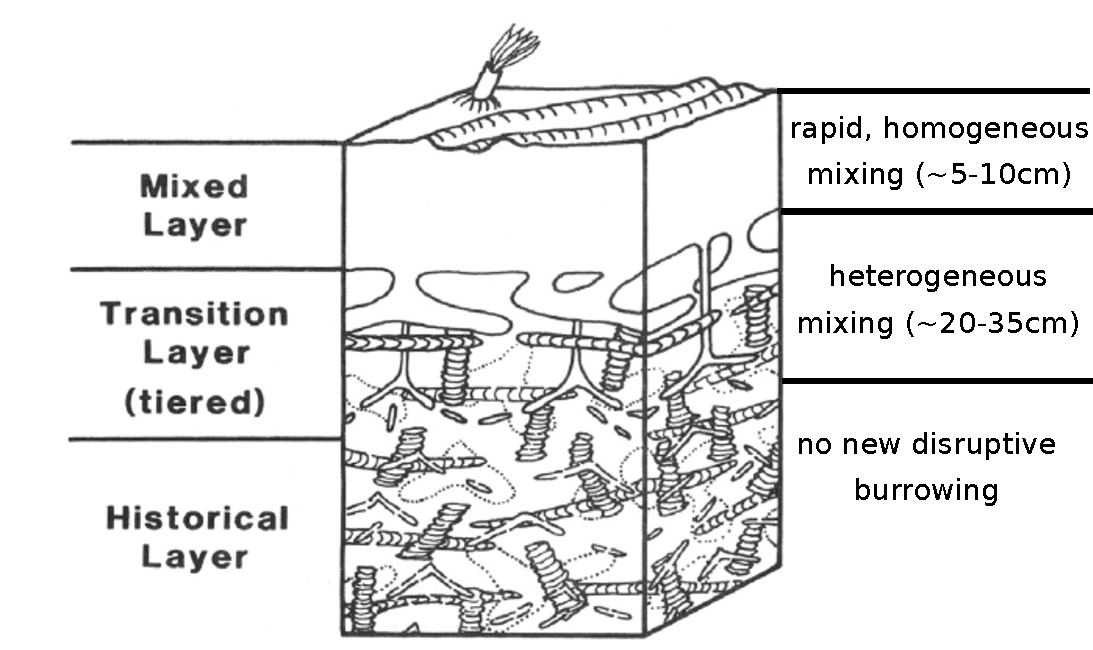
\includegraphics[width=0.6\textwidth]{../figures/Sediment_column.pdf}
	\caption{Copied from  Trauth (2013): Generalized burrow stratigraphy in oxygenated pelagic sediments according
to Savrda et al. (1991) and Savrda (1992). The surface mixed layer (typically 5--10 cm thick) represents an interval of rapid and complete biogenic homogenization.
The transition layer, a zone of heterogeneous mixing that extends to subsurface depths of 20--35 cm, is characterized by burrows produced by organisms that live or
feed at greater depths in the substrate (i.e. below the mixed layer). With continued sediment accretion and associated upward migration of the mixed and transition
layers, sediment passes out of the actively bioturbated zone into a historical layer, in which no new disruptive burrowing takes place. Reprinted without permission of C.V. Svarda.
}\label{fig:TURBO2_schematic}
\end{center}
\end{figure}

\subsection{Experiments:}
In the first set of experiments we simulate the influence of different bioturbation depths (2cm, 5cm, 10cm, 20cm) on abundance and isotopic signals of 2 species. The 
real abundance and the isotopic signal are covaried (e.g. impulse- or stepchange for abundance and isotopic signal at the same time). About 500 total particles (species 1 + 2) are modeled in each layer. 
After mixing, 20 of each foram species are picked in each layer and their isotope values are measured.\\

In the second set of experiments only the isotopic signal in the forams is changed (the magnitude of both species is fixed). Again about 500 total particles are modeled in each layer (now always 350 of species 1 and 150 of species 2). 
After mixing, in order to examine the uncertainties caused by low sample sizes, either 20 or 5 of each foram species are picked in each layer and their isotope values are measured.
Bioturbation depths of 5cm, 10cm and 20cm are used. \\

Each experiment is simulated with 50 different random mixing matrices. Results (abundance and isotope signal) for each single run are plotted in grey. The mean result for the 50 runs is plotted in blue (species 1) and red (species 2).
The black line is the actual change in abundance and isotope signal. The horizontal green line shows the number of carriers which have been measured.

\section{Results}\label{Results} % and model comparison
\subsection{Experiments: Covary abundance and isotope signal}

\begin{figure}[hbp]
\begin{center}
	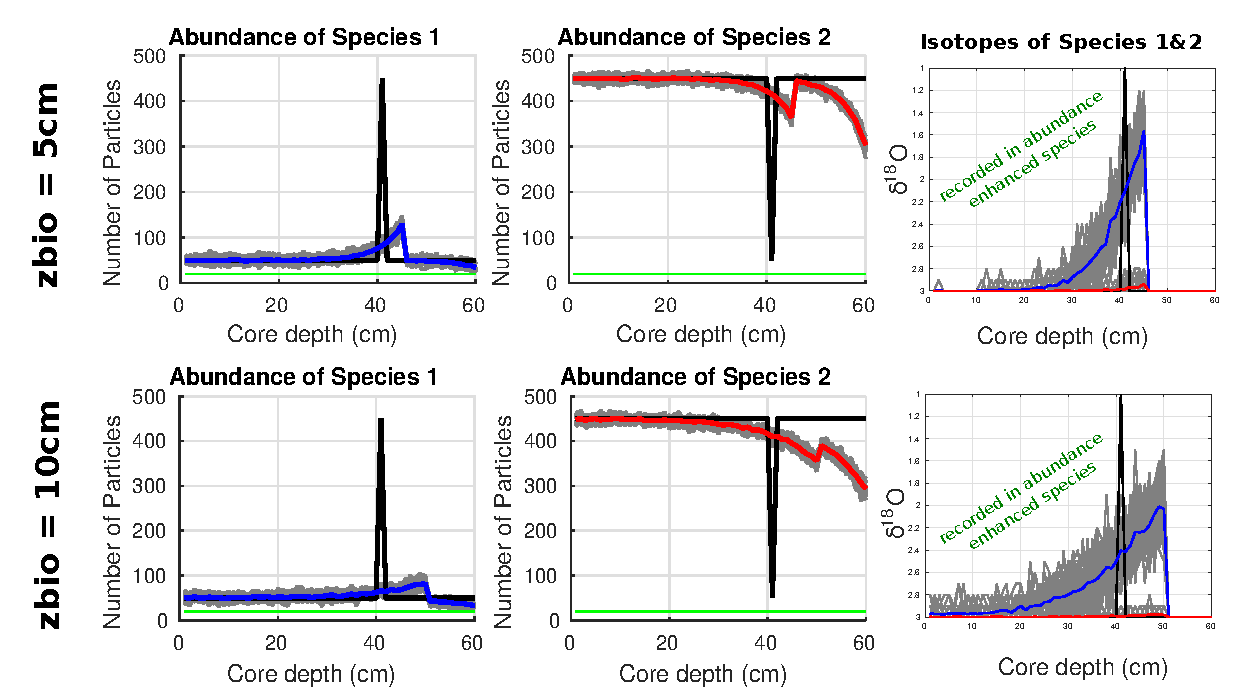
\includegraphics[width=1.0\textwidth]{../figures/1point_event_5+10cm_background.pdf}
	\caption{Mixing of a point/impulse event: Species 1 has an abundance of 50 everywhere except for a single layer that has an abundance of 450 (species 2 is 450 everywhere except in the one layer 50, see black line in left and middle plot). 
	The isotope values also change simultaneously from 3.00\textperthousand\ to 1.00\textperthousand\ for both species (black line in right plots). A constant mixing depth demonstrates the dispersal of the sediment particles over a large depth 
	interval. Highest (lowest) concentrations occur at the base of the mixed layer, i.e. 5 or 10\,cm below their original location. For a deeper mixed layer (i.e. 10cm) the maximum concentration change is smaller. 
	Above that peak the abundance decreases (increases) exponentially. The same trends are observed for the isotope signal - however it is almost only recorded in the abundance enhanced species 1. 
	}\label{fig:1pointevent}
\end{center}
\end{figure}


\begin{figure}[hbp]
\begin{center}
	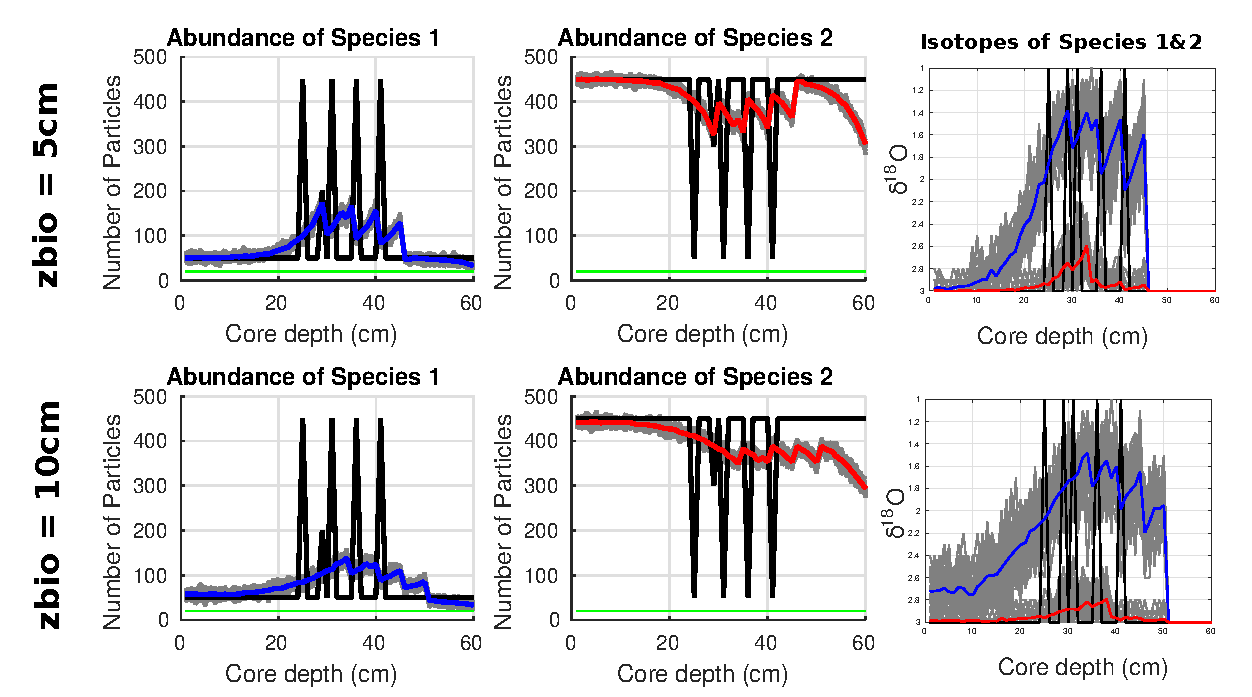
\includegraphics[width=1.0\textwidth]{../figures/../figures/5point_event_5+10cm_background.pdf}
	\caption{Mixing of 5 point/impulse events: All point events have the same abundance change and equal distance except the 4th event which is of smaller magnitude and closer to the previous event. 
	The isotope values again change simultaneously from 3.00\textperthousand\ to 1.00\textperthousand\ for both species. The same horizontal shift in the signals is observed as before but the signals do not recover to background values. 
	Therefore younger observed abundance and isotope changes are more pronounced (especially the smaller 4th perturbation has a similar observed signal).
	For the deeper mixing experiment (z$_\mathrm{bio}=10$cm) the variability in the observed isotope signal is larger (i.e. grey experiments are more distant from the mean).
}\label{fig:5pointevent}
\end{center}
\end{figure}


\begin{figure}[hbp]
\begin{center}
	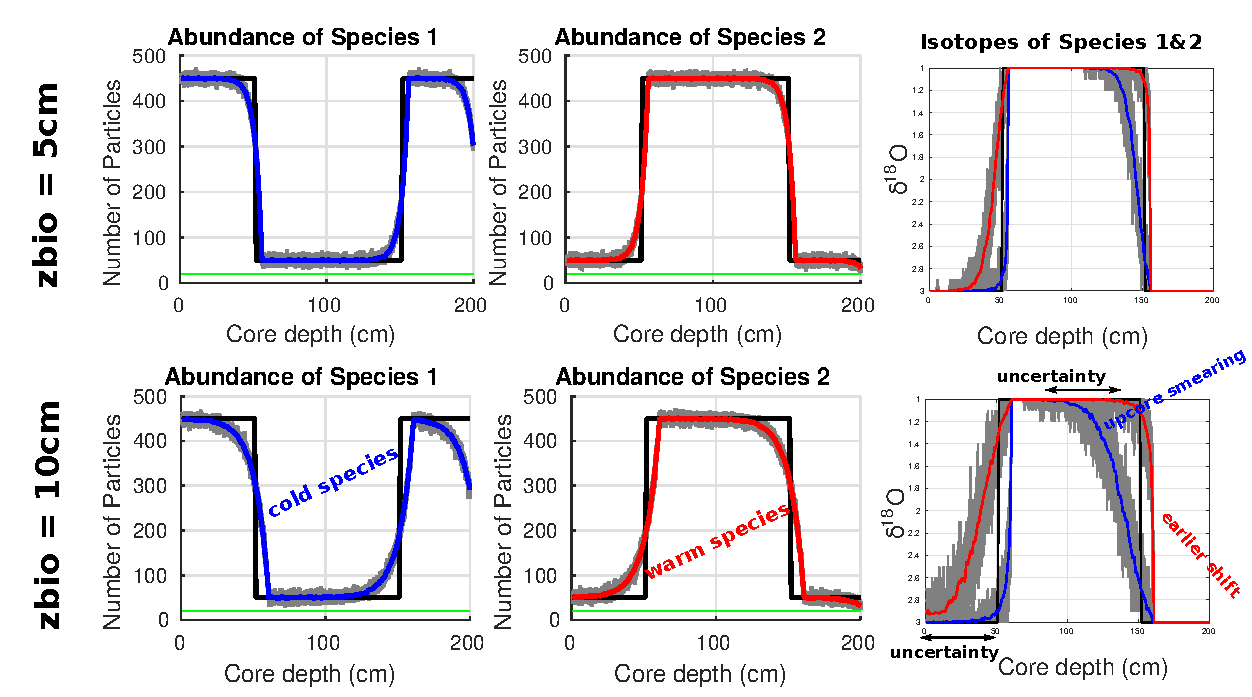
\includegraphics[width=1.0\textwidth]{../figures/../figures/stepchange2_5+10cm_background.pdf}
	\caption{Mixing of a step change: Impact of homogenized mixing of the top 5 and 10 cm of sediment on an abrupt change in the abundance of a foraminifera species in the middle of a sequence, 
	from 450 individuals (species 1) to 50 individuals and back (isotope values change simultaneously). \\
	Adapted from Trauth (2013): The original shift (warming) in climate, documented by the change from heavy (3.00\textperthousand\ ) to light (1.00\textperthousand\ ) isotope values, occurs at 150 cm depth, whereas the warm
	species (Species 2) already documents this shift at $\sim 160$ cm depth; the isotope record from the cold species (Species 1), however, shows a broad transition band between $\sim 160$ and $\sim 90$ cm core depth (z$_\mathrm{bio}=10$cm).
	The phase difference of more than $\sim 50$cm between the isotope records from the two species, which both experienced the same change in climate during deposition of the sediment layer (at 150 cm depth), 
	can result in dramatic uncertainties when developing an oxygen isotope stratigraphy for this type of deep sea core.
}\label{fig:stepchange}
\end{center}
\end{figure}


\begin{figure}[hbp]
\begin{center}
	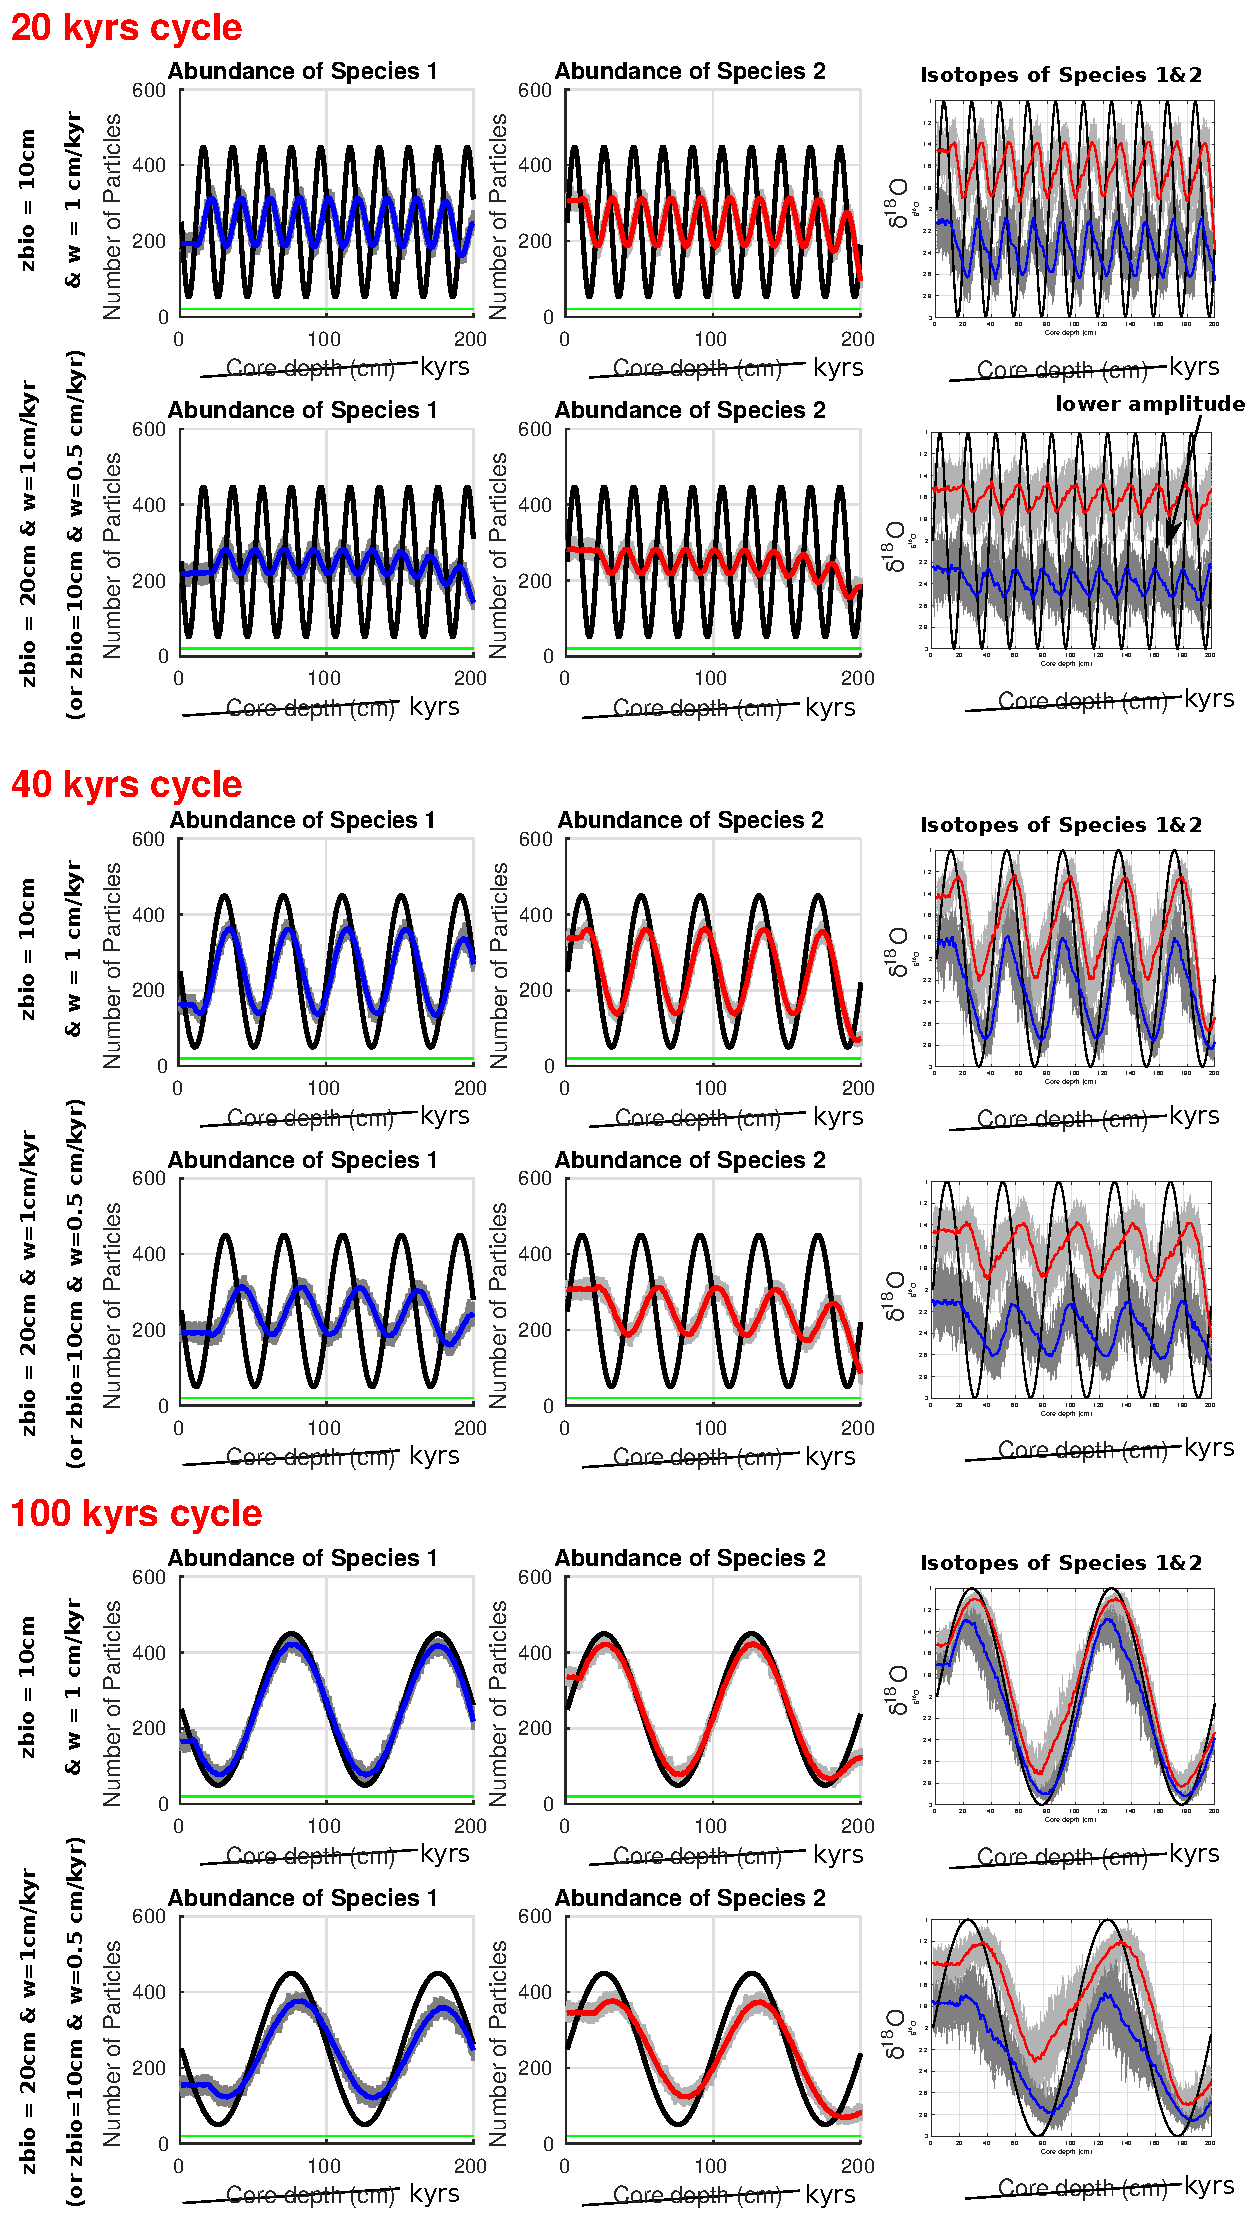
\includegraphics[width=0.7\textwidth]{../figures/../figures/20+40+100kyrcycle_10+20cm_background.pdf}
	\caption{Mixing of cycles (sine waves): Abundance of species 1 and 2 and the isotope signal is changed with different periodicities. Core depth can now be translated in age. A change in z$_\mathrm{bio}$ with fixed sedimentation rate ($w$) 
	gives the same results as a change in sedimentation rate with fixed z$_\mathrm{bio}$ (e.g. z$_\mathrm{bio}=20cm$ \& $w=1$ cm/kyr equals z$_\mathrm{bio}=10cm$ \& $w=0.5$ cm/kyr).\\
	Deeper bioturbation (or lower sedimentation rate) results in a lower amplitude of the observed abundance and isotope signal especially in the 20 kyr cycle. 
	}\label{fig:sine-waves}
\end{center}
\end{figure}


\begin{figure}[hbp]
\begin{center}
	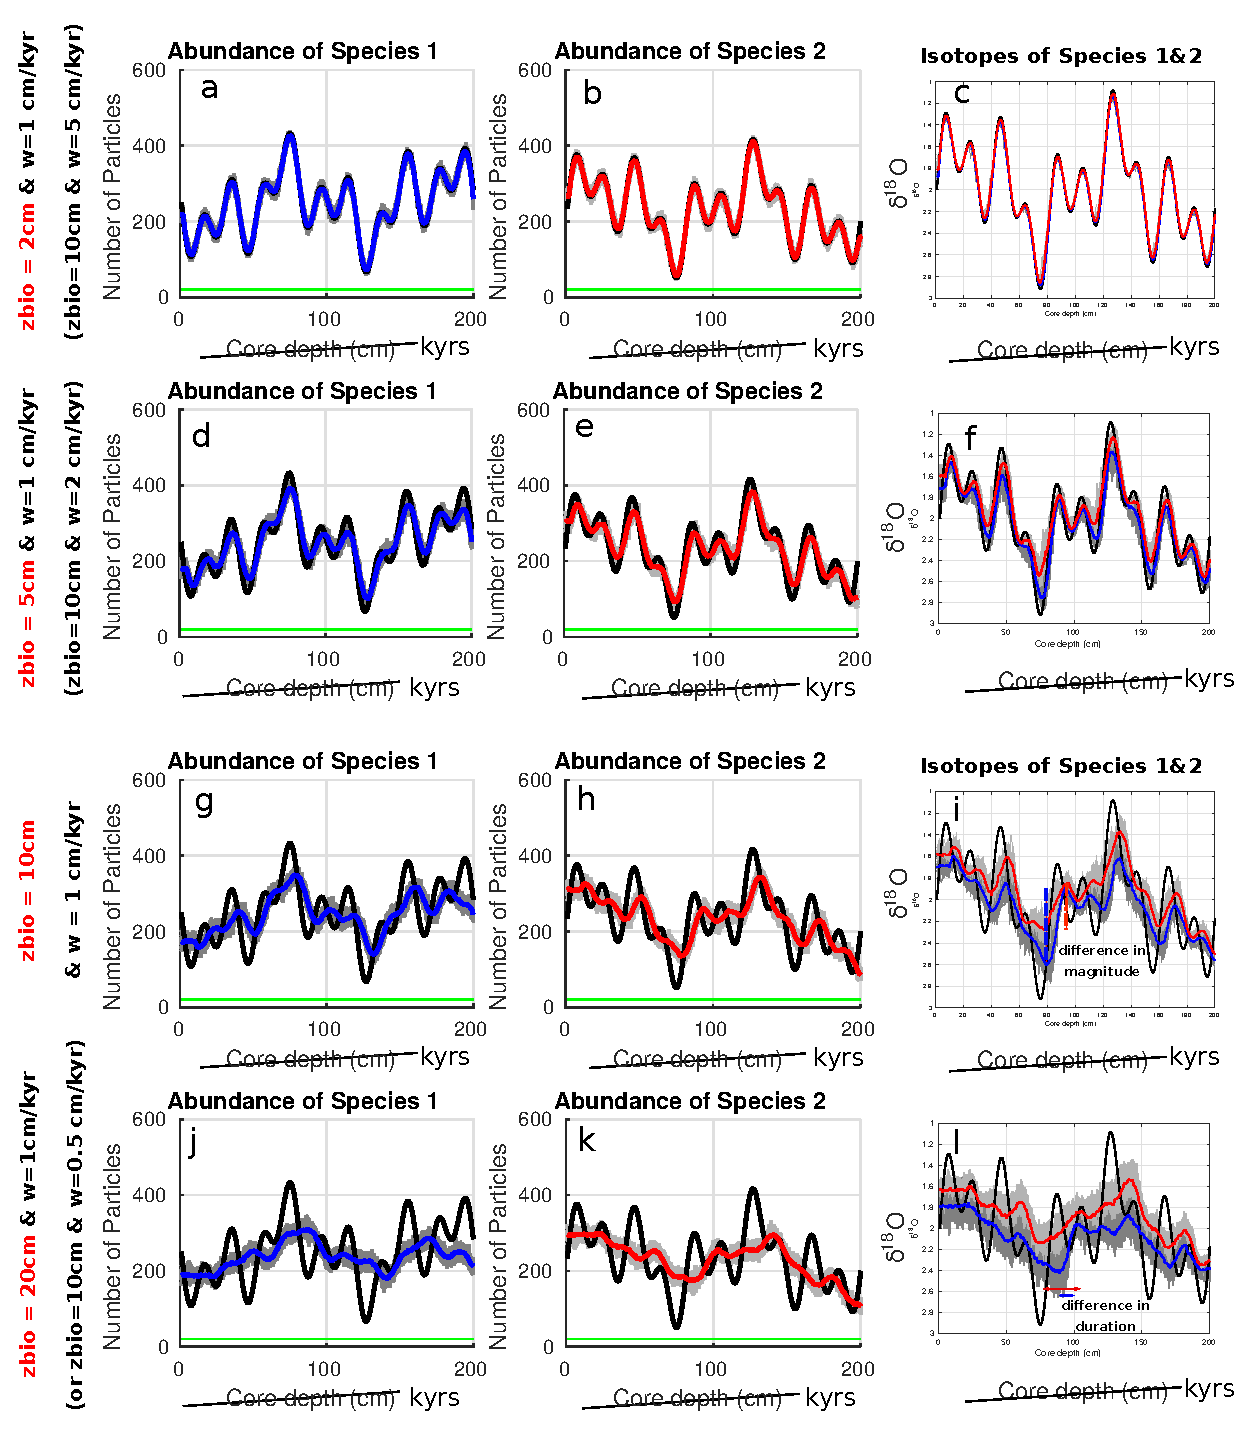
\includegraphics[width=0.8\textwidth]{../figures/../figures/Allcycles_combined_2+5+10+20cm_background.pdf}
	\caption{Mixing of the three combined cycles (20, 40 and 100 kyrs) with z$_\mathrm{bio} \in \{2,5,10,20 \}$cm. Abundance of species 1 and 2 and the isotope signal is changed simultaneously. 
	A mixed layer of 2 cm has no effect on the observed isotope signal of both species. For z$_\mathrm{bio}\geq=10cm$ the isotope records from the two species (which both experienced the same change) show discrepancies 
	in both the magnitude (i) and the duration (l) of the change.}\label{fig:allcyclescombined}
\end{center}
\end{figure}


\begin{figure}[hbp]
\begin{center}
	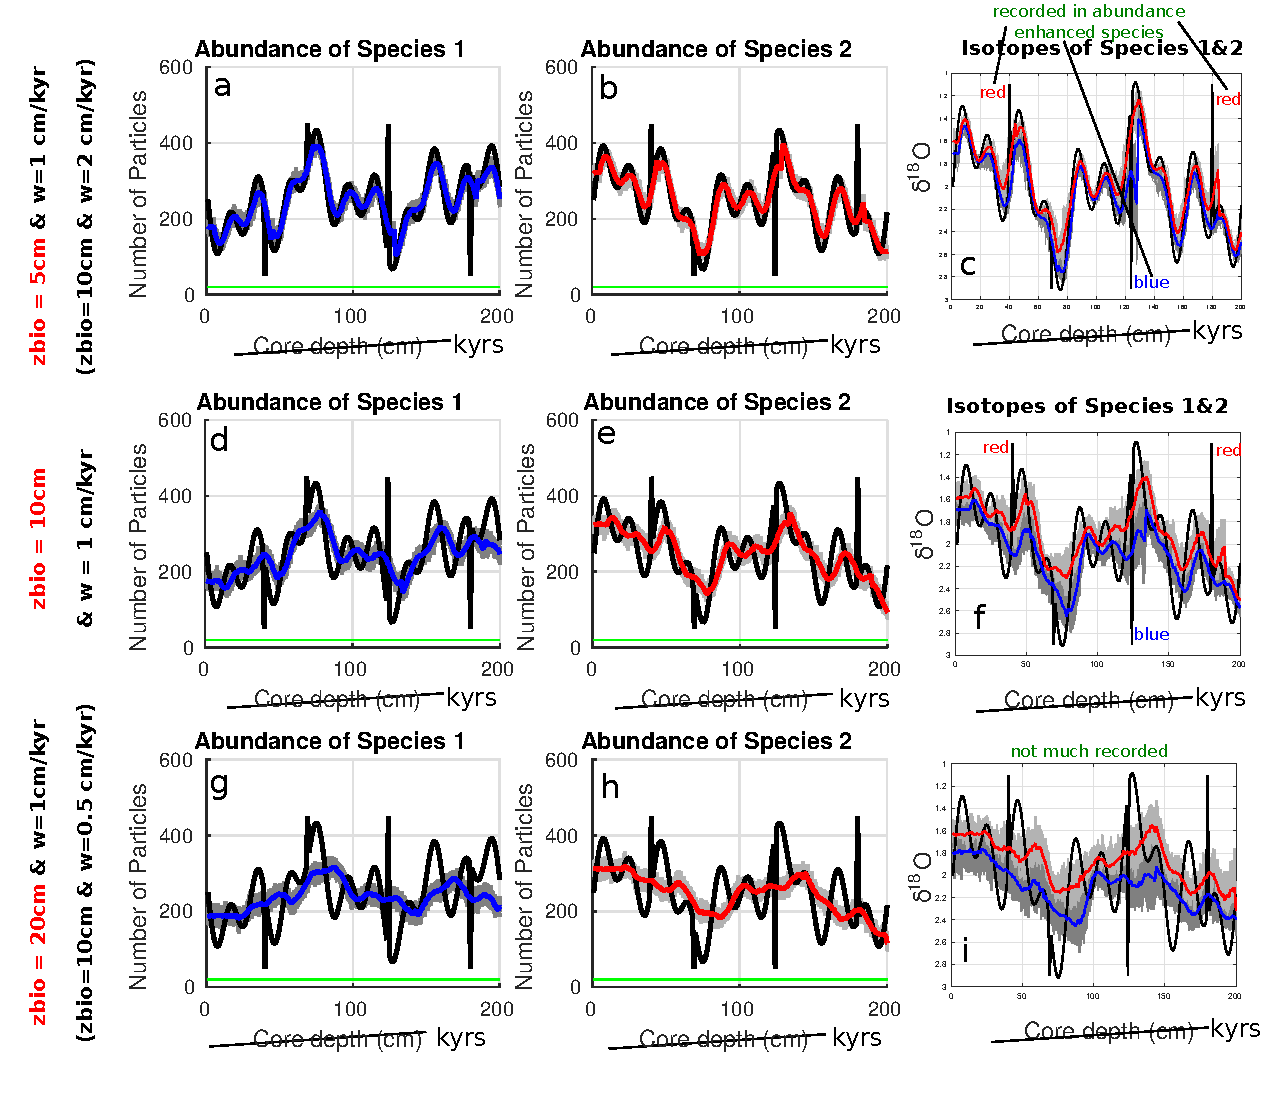
\includegraphics[width=1.0\textwidth]{../figures/../figures/Allcycles_combined_pointevent_5+10+20cm_background.pdf}
	\caption{Mixing of the three combined cycles (20, 40 and 100 kyrs) with z$_\mathrm{bio} \in \{5,10,20 \}$cm. Abundance of species 1 and 2 and the isotope signal is changed simultaneously. Additionaly we change the abundance and isotope signal 
	in discrete pulse events. Only the isotope record of the abundance enhanced species shows the pulse event (c, f). However, if the mixed layer is very deep (z$_\mathrm{bio}\geq=20cm$) the pulse event is not visible anymore (i).}\label{fig:allcycles+pointevent}
\end{center}
\end{figure}
\begin{figure}[hbtp]
\hspace*{-0.8cm}%\caption{Observations from}
\end{figure}

\begin{figure}[hbp]
\begin{center}
	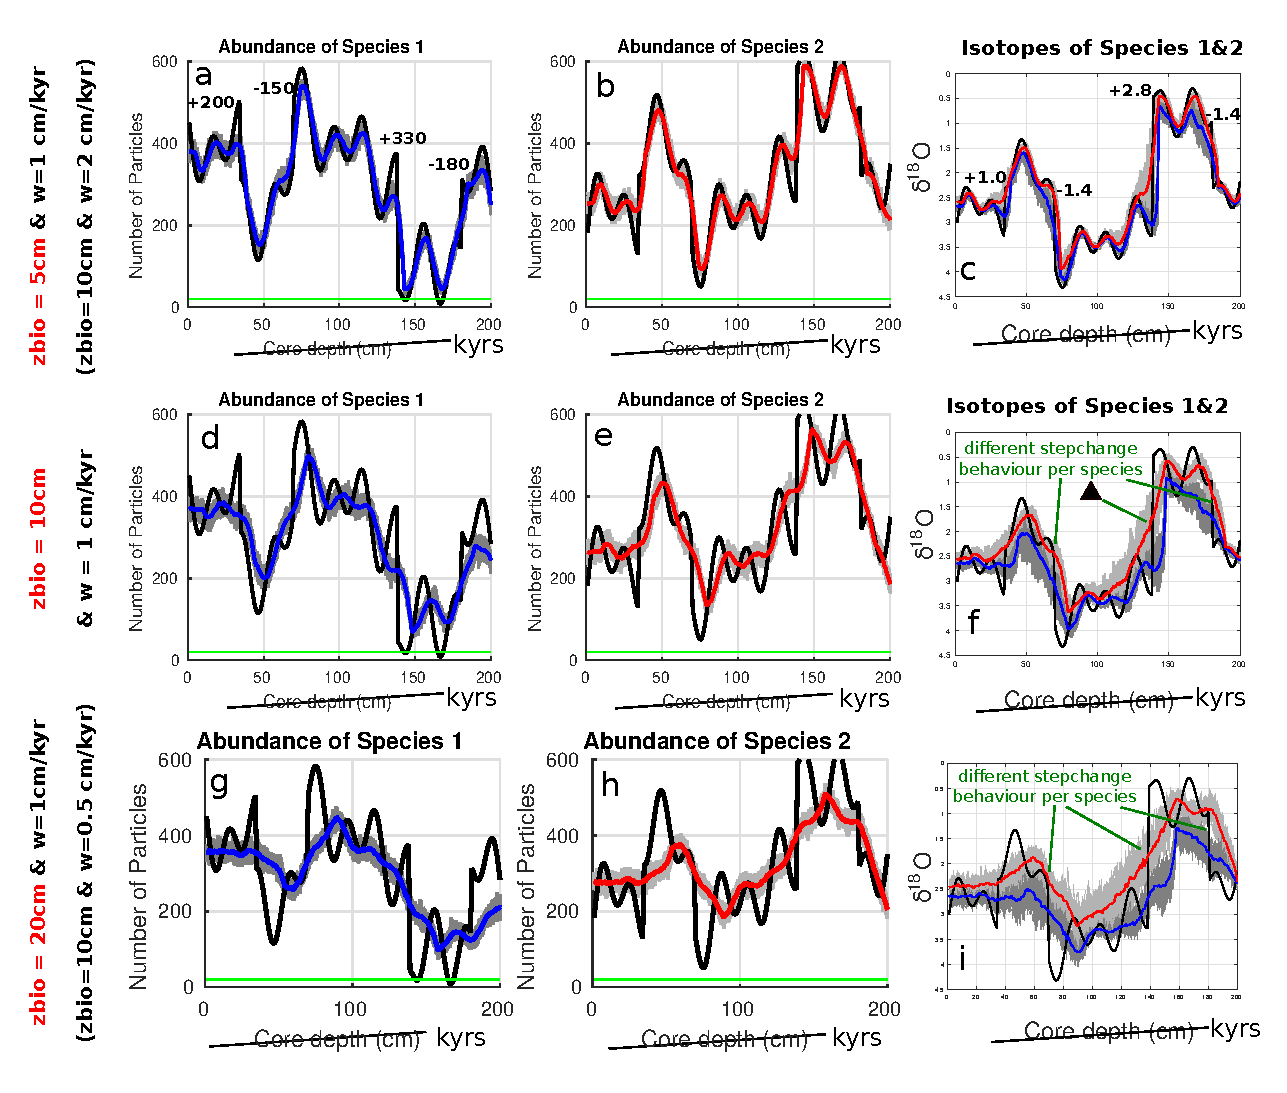
\includegraphics[width=1.0\textwidth]{../figures/../figures/Allcycles_combined_stepevent_bigger_5+10+20cm_background.pdf}
	\caption{Mixing of the three combined cycles (20, 40 and 100 kyrs) with z$_\mathrm{bio} \in \{5,10,20 \}$cm. Abundance of species 1 and 2 and the isotope signal is changed simultaneously. Additionaly we change the abundance and isotope signal 
	at various steps (black numbers in a, c). Results show different step change behavior for the isotope record in the two species -- the abundance enhanced species documents the respective shift early on and as a rapid shift 
	(e.g. blue at $\blacktriangle$ in f) whereas the isotope shift in the shrinking species is much broader and slower (e.g. red at $\blacktriangle$ in f).}\label{fig:5pointevent}
\end{center}
\end{figure}


\newpage
\subsection{Experiments: Only change isotope signal - fixed abundance}
Only the isotopic signal in the forams is changed (same magnitude in both species). Again about 500 total particles are modeled in each layer (now always 350 of species 1 and 150 of species 2). 
After mixing, in order to examine the uncertainties caused by low sample sizes, either 20 or 5 of each foram species are picked in each layer and their isotope values are measured.
Bioturbation depths of 5cm, 10cm and 20cm are used. 

\begin{figure}[hbp]
\begin{center}
	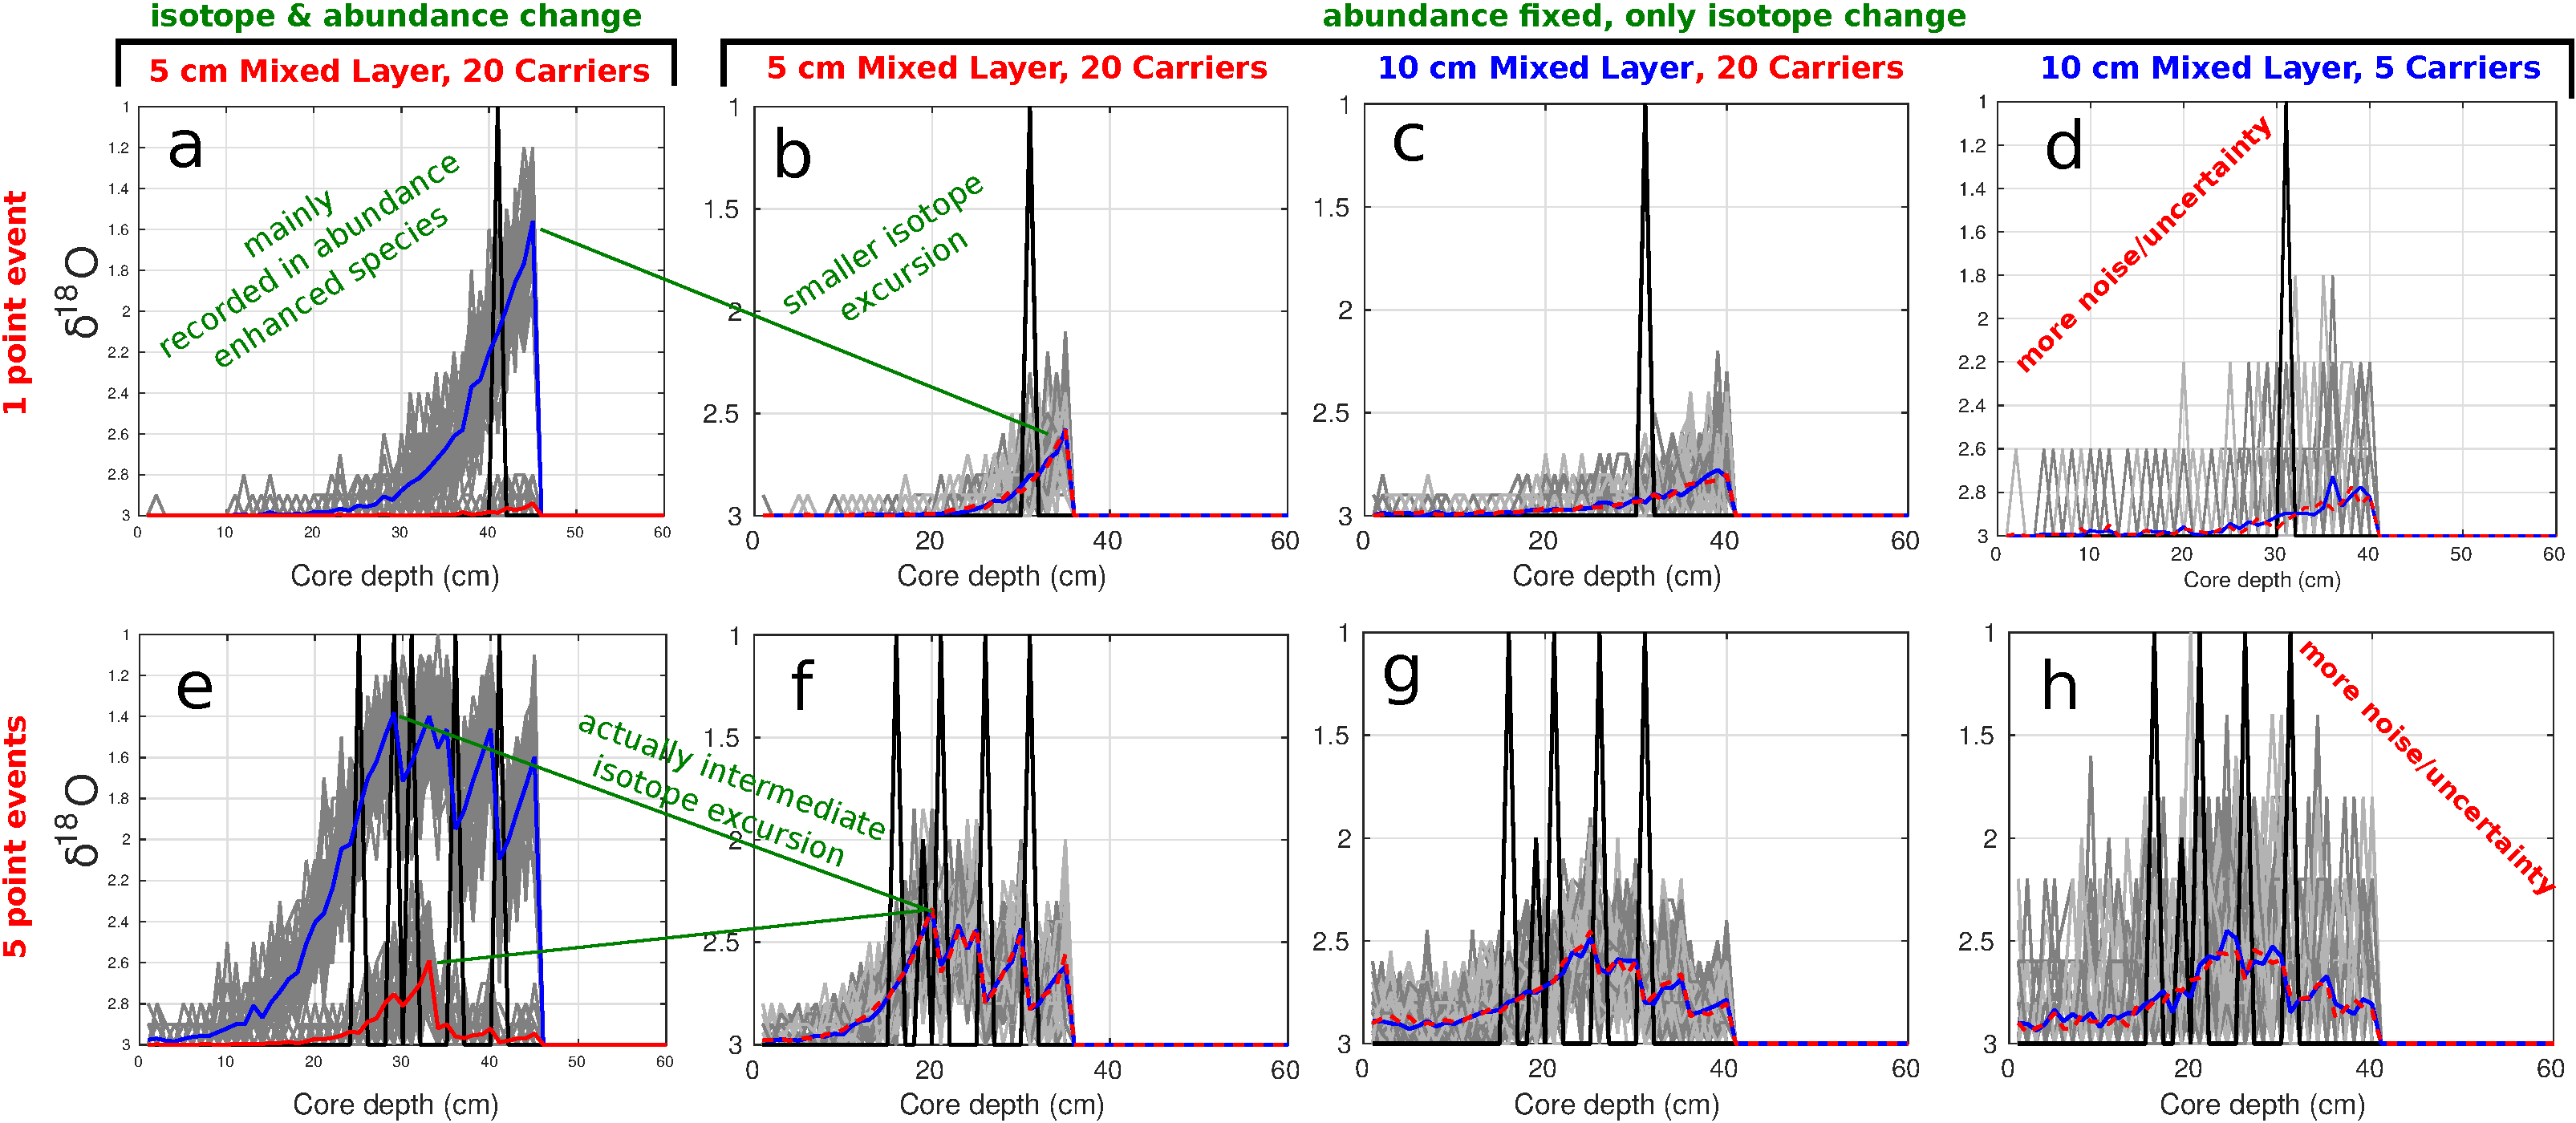
\includegraphics[width=1.0\textwidth]{../figures/../figures/JustABU_pointevent1+5.pdf}
	\caption{Example: Step changes - all cycles combined with z$_\mathrm{bio} \in \{5,10\}$cm and sample size of 20 and 5. }\label{fig:5pointevent}
\end{center}
\end{figure}



\begin{figure}[hbp]
\begin{center}
	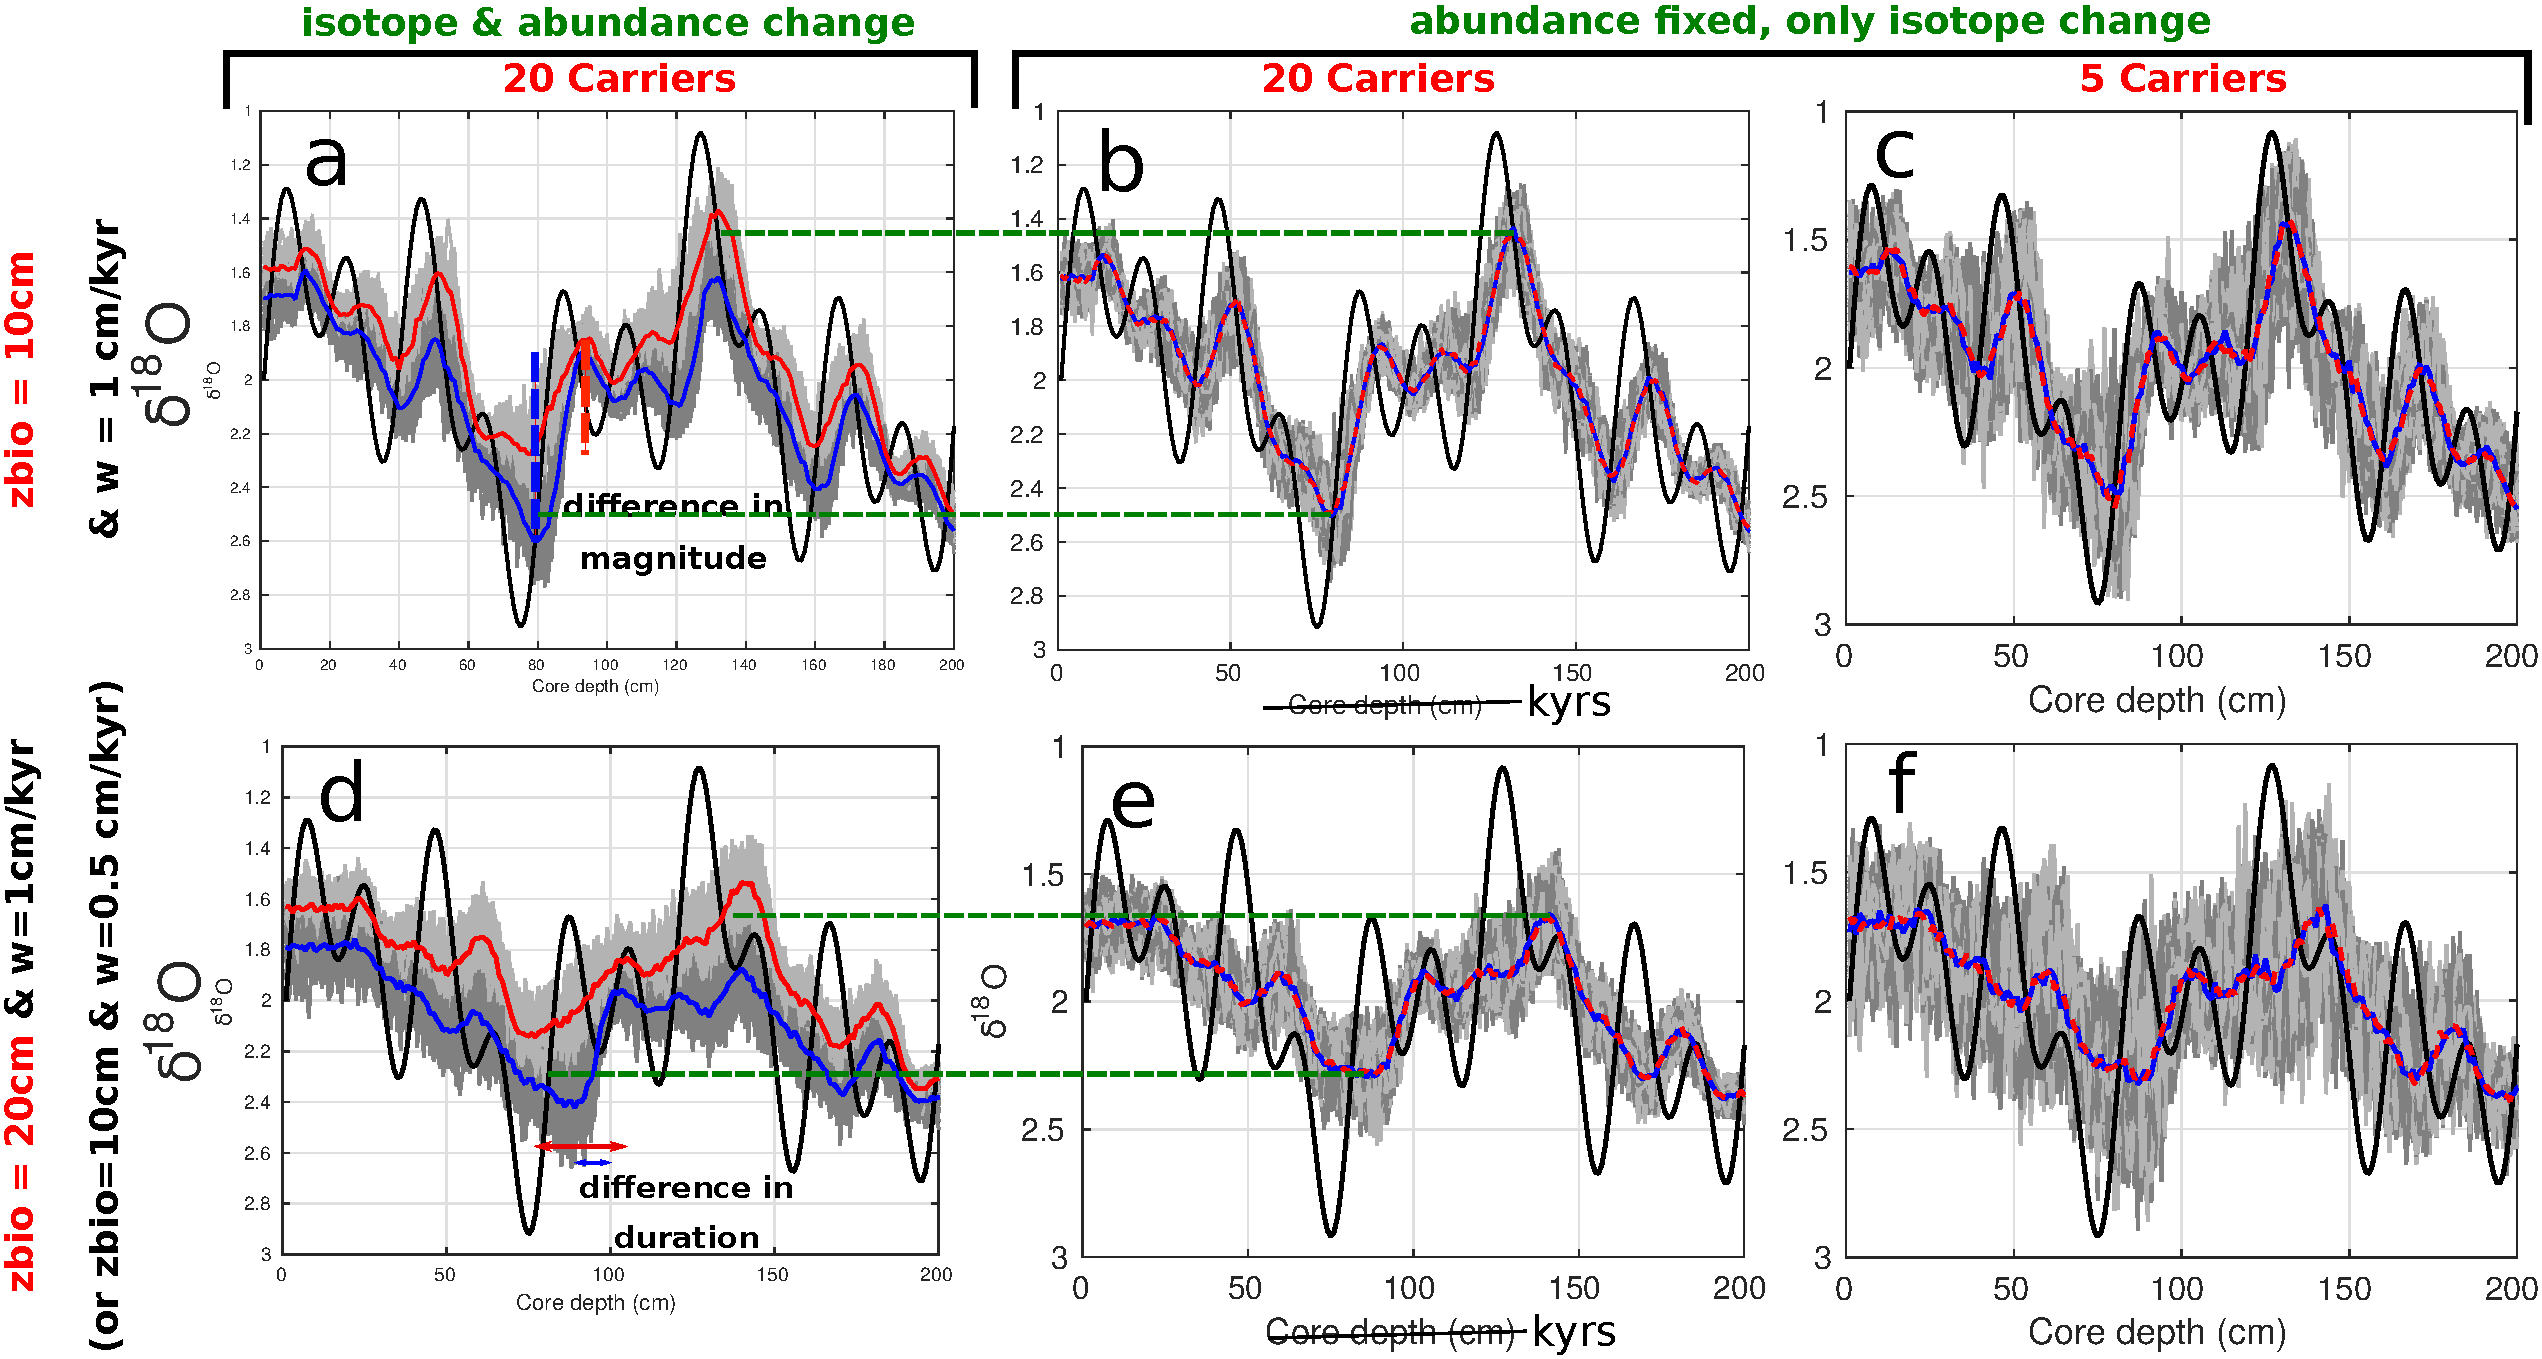
\includegraphics[width=1.0\textwidth]{../figures/../figures/JustABU_3ycles_combined.pdf}
	\caption{Example: All cycles combined with z$_\mathrm{bio} \in \{10,20 \}$cm and sample size of 20 and 5. }\label{fig:5pointevent}
\end{center}
\end{figure}

\begin{figure}[hbp]
\begin{center}
	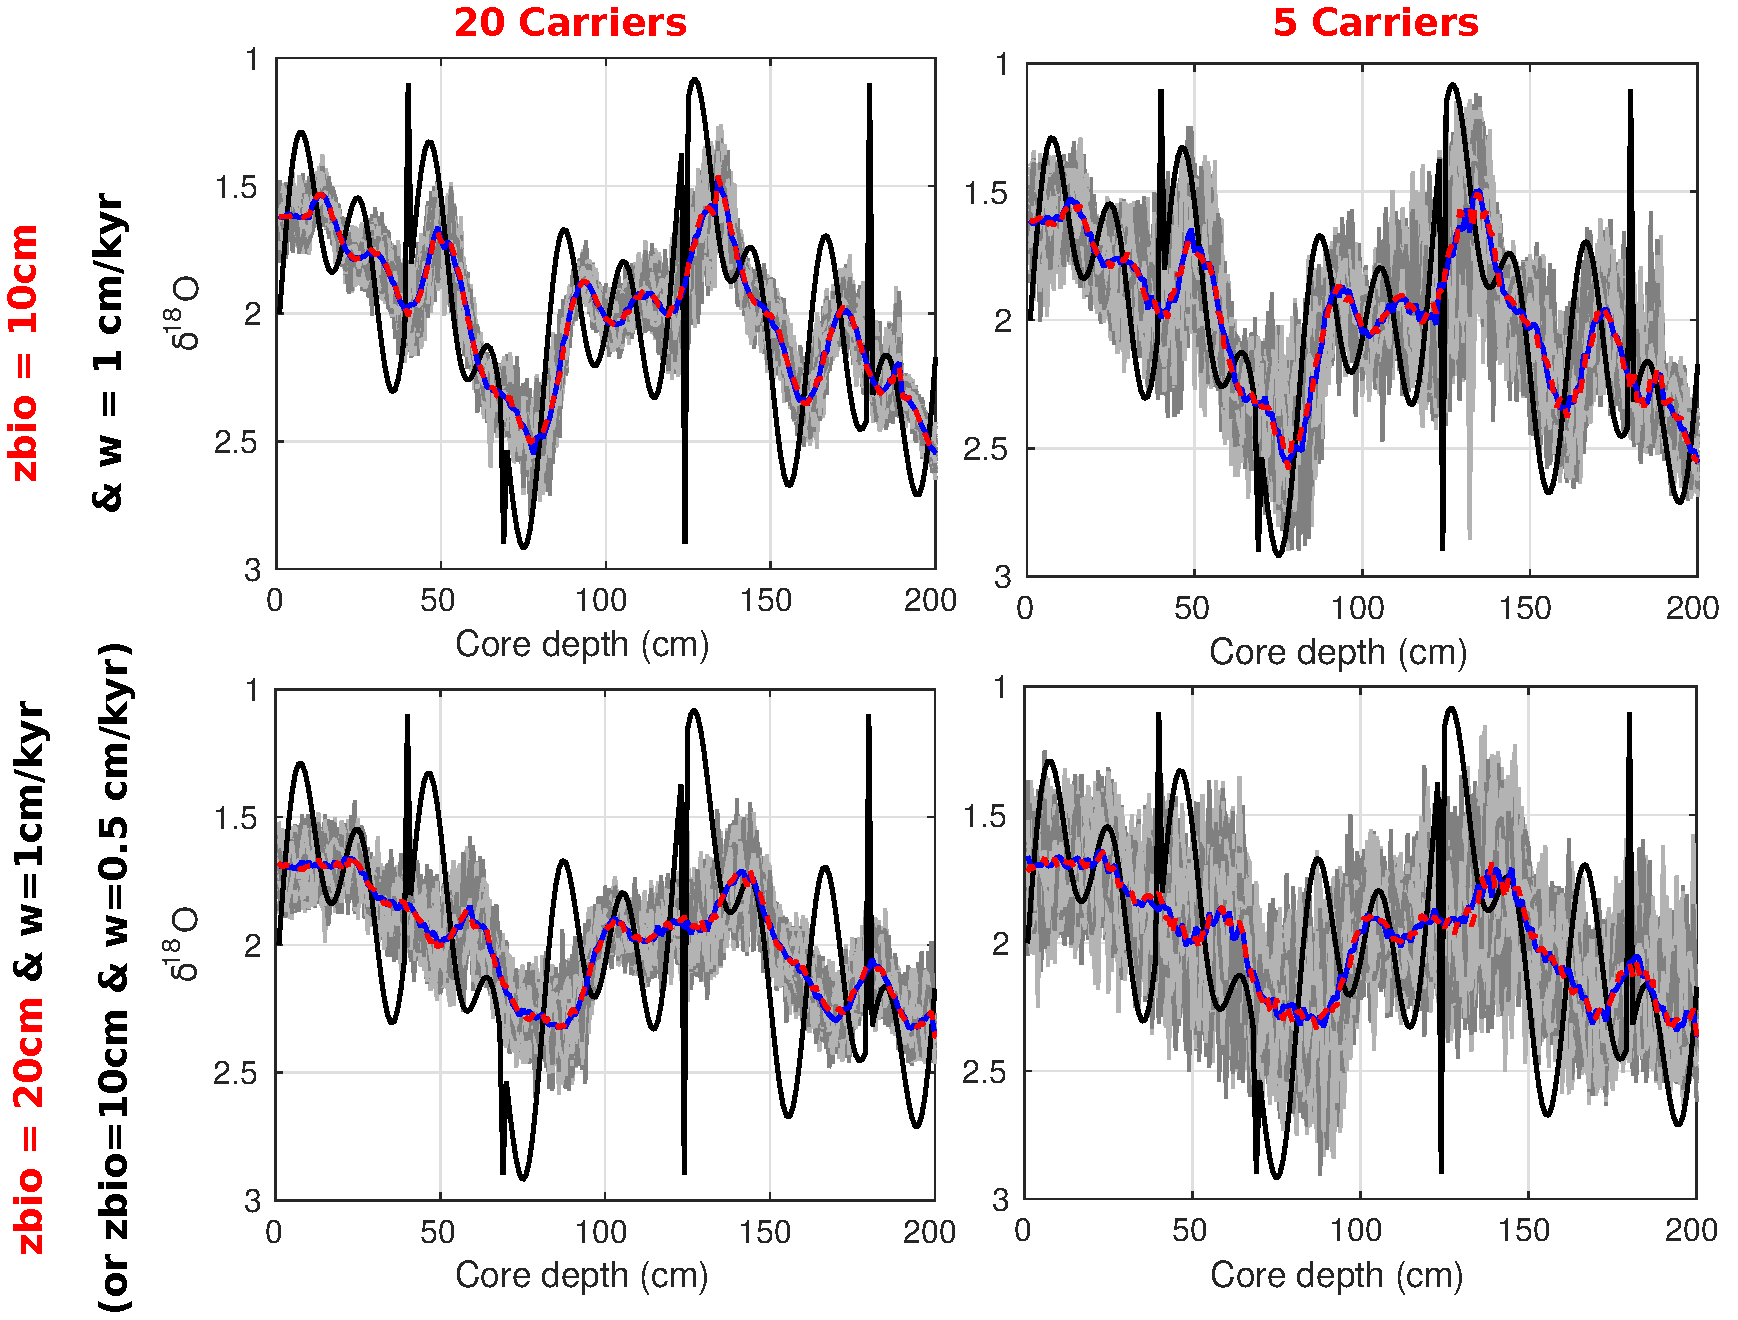
\includegraphics[width=1.0\textwidth]{../figures/../figures/JustABU_3ycles_combined_pointevents.pdf}
	\caption{Example: Point events - all cycles combined with z$_\mathrm{bio} \in \{10,20 \}$cm and sample size of 20 and 5. }\label{fig:5pointevent}
\end{center}
\end{figure}

\begin{figure}[hbp]
\begin{center}
	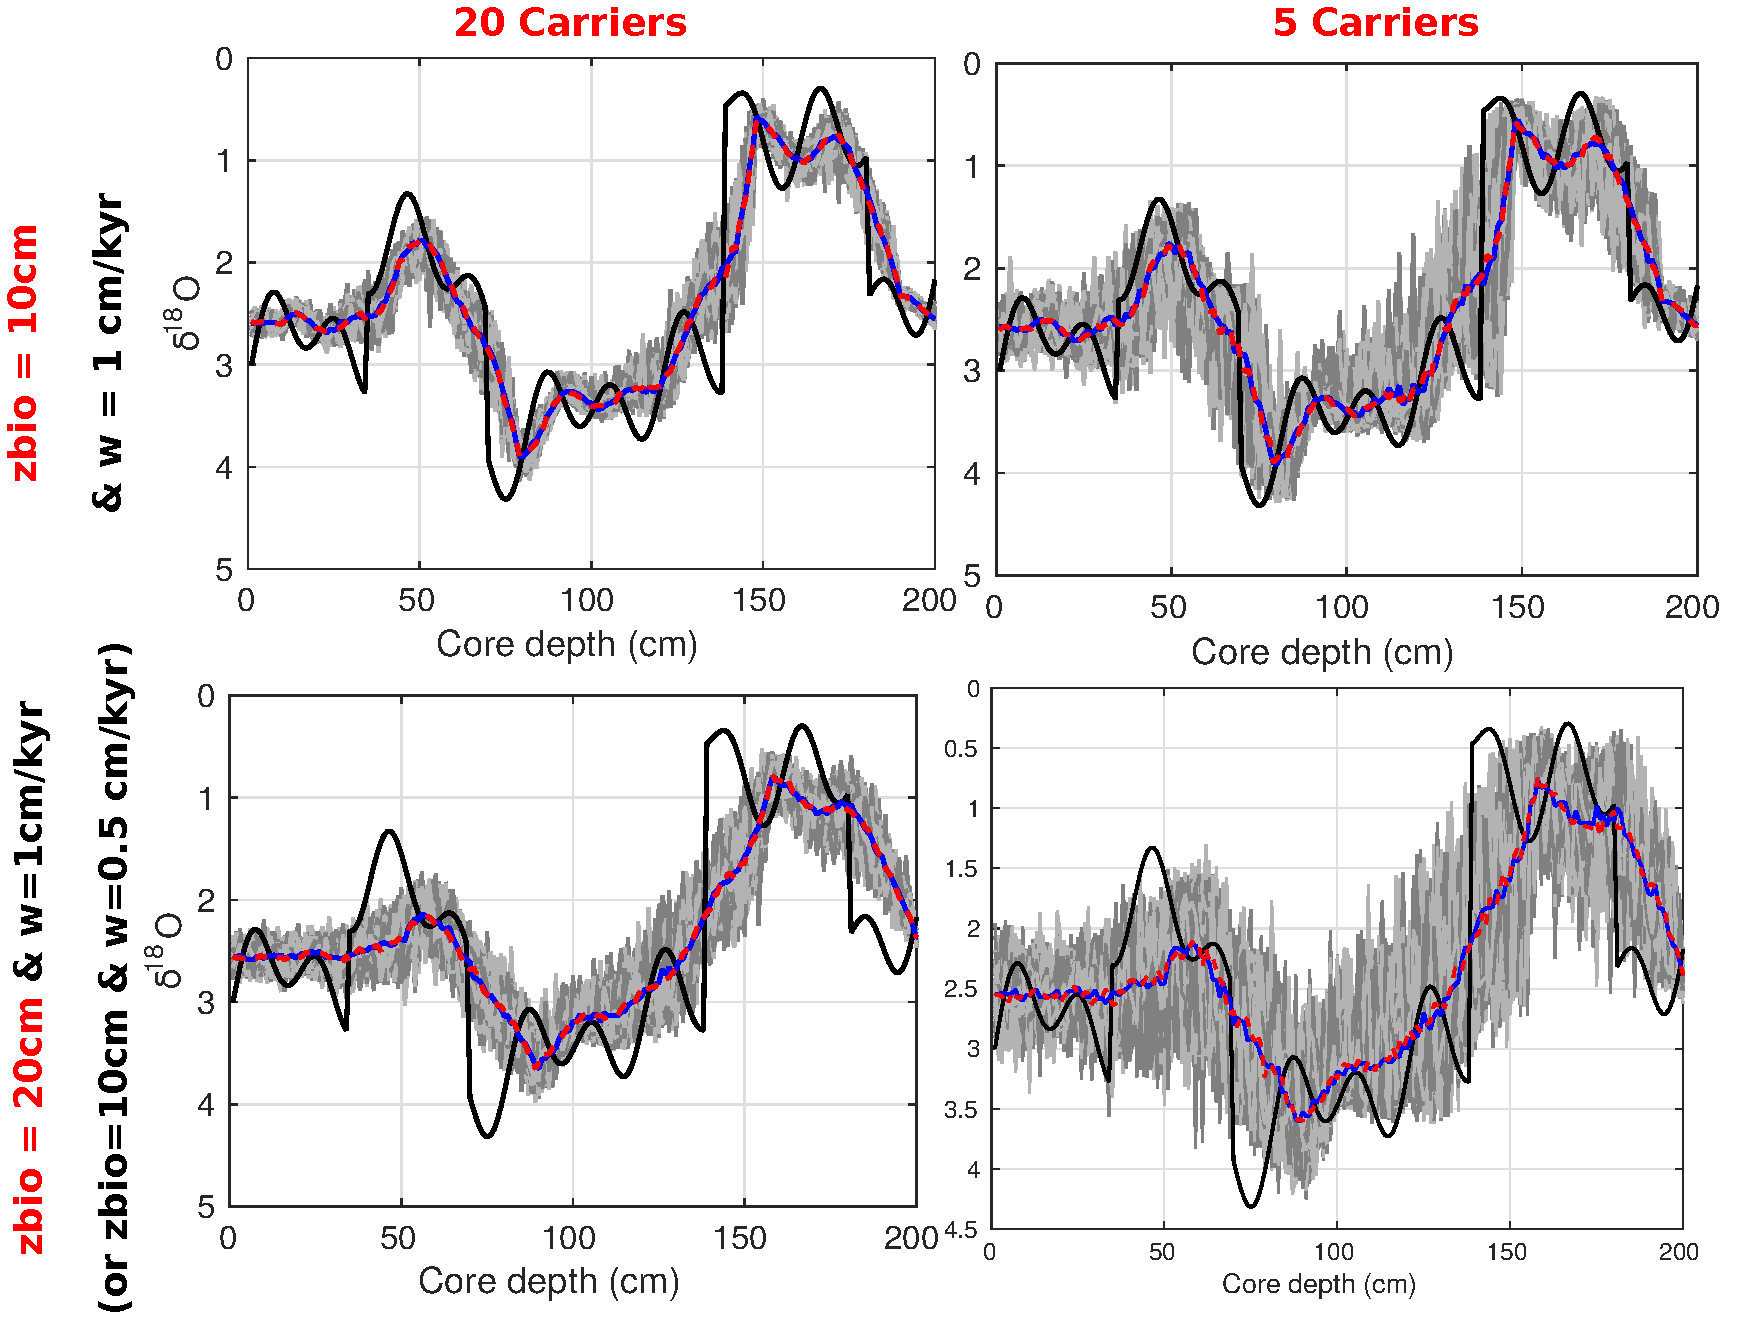
\includegraphics[width=1.0\textwidth]{../figures/../figures/JustABU_3ycles_combined_gradual.pdf}
	\caption{Example: Step changes - all cycles combined with z$_\mathrm{bio} \in \{10,20 \}$cm and sample size of 20 and 5. }\label{fig:5pointevent}
\end{center}
\end{figure}
\newpage
%% The Bibliography
%% ==> You need a file 'literature.bib' for this.
%% ==> You need to run BibTeX for this (Project | Properties... | Uses BibTeX)
%\addcontentsline{toc}{chapter}{Bibliography} %'Bibliography' into toc
%\nocite{*} %Even non-cited BibTeX-Entries will be shown.

% \bibliographystyle{apalike} %Style of Bibliography: plain / apalike / amsalpha / ...
% %\bibliography{/home/alex/BRL/bib/literature/VORbib.bib} %You need a file 'literature.bib' for this.
% \bibliography{TURBO_050618}


\end{document}
